\chapter{Transfer Function}
\label{chap:tf}
The transfer function was calculated from the system equation
\eqref{eq:equationmotion} analysed in the section
\ref{subsec:equationofomotion}.
%
\begin{equation}
\label{eq:gs}
	G(s) = \big([M]s^2+[C]s+[K]\big)^{-1}
\end{equation}
%
Given \(F(s) = g_{\text{v}}V(s)\)  the Laplace transform of the force signal,
thus the transfer function can be write:
\begin{align}
\label{eq:tf}
  {X(s)} &= G(s)\frac{F(s)}{g_{\text{v}}}\\
  \frac{X(s)}{F(s)} &= \frac{1}{g_{\text{v}}}\,{G(s)}
\end{align}
%
\begin{figure}[htb]
	\centering
	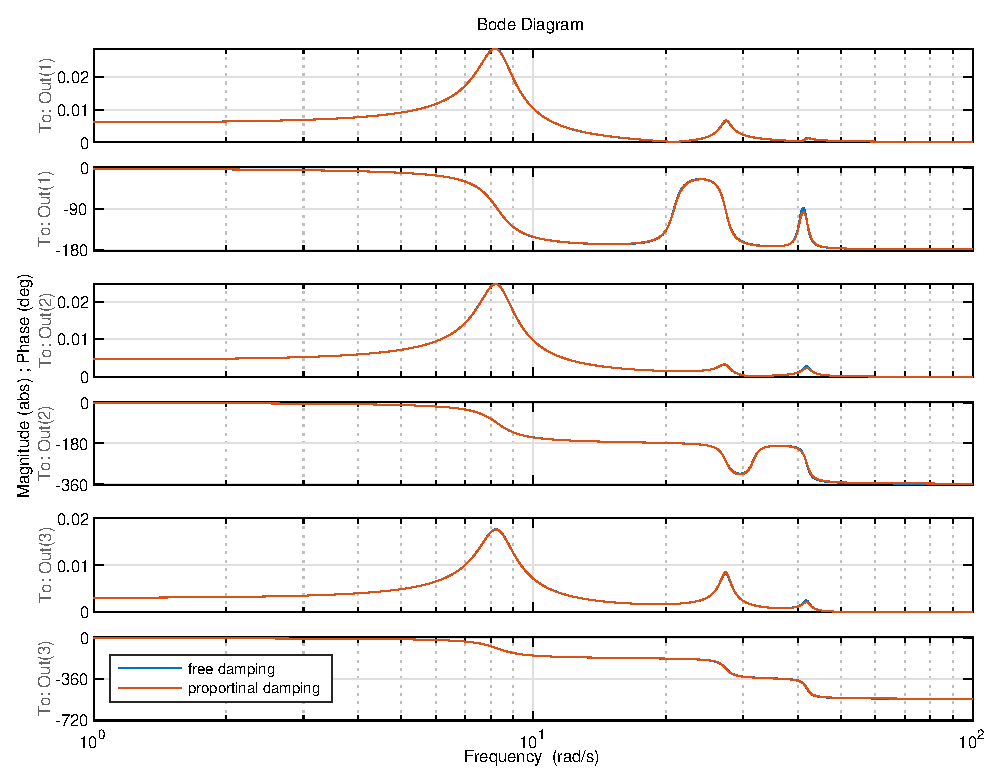
\includegraphics[width=0.66\textwidth]{bodediagram1}
	\caption{Bode diagram of the transfer functions as in \eqref{eq:tf}}
	\label{fig:bodeplot1}
\end{figure}
%
The bode diagram are shown in Figure \ref{fig:bodeplot1}.